\documentclass{beamer}
%------------------------------------------
\usecolortheme{rose}
%------------------------------------------
\useinnertheme{circles}
%------------------------------------------
\setbeamertemplate{navigation symbols}{}
%------------------------------------------
\AtBeginSection{
    \begin{frame}<beamer>\small
        \tableofcontents[currentsection,subsectionstyle=shaded/shaded/hide]
    \end{frame}
}
%------------------------------------------
\AtBeginSubsection{	
    \begin{frame}<beamer>\small
        \tableofcontents[
            currentsection,sectionstyle=shaded/shaded,
            currentsubsection,subsectionstyle=show/shaded/hide]
    \end{frame}
}
%------------------------------------------
\usepackage[overridenote]{pdfpc}

\usepackage{tikz}
\usetikzlibrary{
    % shapes,
    % arrows,
    % backgrounds,
    positioning,
}
\tikzset{
    sm/.style={
        rectangle,
        rounded corners,
        fill=teal!10,
        align=center,
        minimum height=1.5em,
        },
    sup/.style={
        rectangle,
        rounded corners,
        fill=blue!10,
        align=center,
        minimum height=1.5em,
        },
    sub/.style={
        rectangle,
        rounded corners,
        fill=red!10,
        align=center,
        minimum height=1.5em,
        },
    ind/.style={
        align=center,
        minimum height=1.5em,
        },
}

\usepackage[T1]{fontenc}
\usepackage{hyperref}
\hypersetup{%
  colorlinks=true,
  allcolors=blue,
}
\usepackage{commath}
\usepackage{amssymb}
%
% Local commands
%
\newcommand{\todo}[1]{{\color{orange}TODO #1}}
\newcommand{\naf}{\ensuremath{\sim\!}}
\newcommand{\larr}{\ensuremath{\leftarrow}}
\newcommand{\at}[1]{\ensuremath{\!\del{#1}}}
\newcommand{\co}[1]{\ensuremath{\overline{#1}}}
\newcommand{\fml}[1]{\ensuremath{{\cal #1}}}
\newcommand{\deft}[1]{\textbf{#1}}
\newcommand{\pset}[1]{\ensuremath{\mathbb{P}\at{#1}}}
\newcommand{\ent}{\ensuremath{\lhd}}
\newcommand{\cset}[2]{\ensuremath{\set{#1,~#2}}}
\newcommand{\langof}[1]{\ensuremath{\fml{L}\at{#1}}}
\newcommand{\uset}[1]{\ensuremath{\left|{#1}\right>}}
\newcommand{\lset}[1]{\ensuremath{\left<{#1}\right|}}
\newcommand{\pr}[1]{\ensuremath{\mathrm{p}\at{#1}}}
\newcommand{\given}{\ensuremath{~\middle|~}}
%
%	Identificação deste documento
%
\title{Zugzwang}
\subtitle{Stochastic Adventures in Inductive Logic}
\author{Francisco Coelho}
\institute[\texttt{fc@uevora.pt}]{
  Departamento de Informática, Universidade de Évora\\
  High Performance Computing Chair\\
  NOVA-LINCS
}

\begin{document}
%
\begin{frame}[plain]
\titlepage
\end{frame}

\section{Introduction}


\begin{frame}{Notation and Assumptions}
    % --------------------------------
    \begin{itemize}
        % --------------------------------
        \item $\co{x} = 1 - x$.
        % --------------------------------
        \item \textbf{Probabilistic Atomic Choice (PAC):} $x :: a$ defines $a \lor \neg a$ and probabilities $\pr{a} = x, \pr{\neg a} = \co{x}$. 
        % --------------------------------
        \item $\delta a$ denotes $a \lor \neg a$ and $\delta\! \set{x :: a, a \in \fml{A}} = \set{\delta a, a \in \fml{A}}$ for a set of atoms $\fml{A}$.
        % --------------------------------
        \item \textbf{Closed World Assumption:} $\naf p \models \neg p$.
        % --------------------------------
        % \item Probabilistic choices and sub-goals are independent.
        % --------------------------------
    \end{itemize}
    % --------------------------------
\end{frame}
% ================================================================
\begin{frame}{General Setting}
    % --------------------------------
    \begin{itemize}    
        % --------------------------------
        \item  \textbf{Atoms} $\fml{A}$,
        $\overline{\fml{A}} = \cset{\neg a}{a \in \fml{A}}$, and \textbf{literals} $\fml{L} = \fml{A} \cup \co{\fml{A}}$.
        % --------------------------------
        \item \textbf{Samples} $z \in  \fml{Z} \iff z \subseteq \fml{L}$.
        % --------------------------------
        \item \textbf{Events} or \textit{consistent samples} $\fml{E}$ :
        $$\fml{E} = \cset{z \in \fml{Z} }{ \forall a \in \fml{A}~\envert{\set{a,\neg a} \cap z} \leq 1}.$$
        % --------------------------------
        \item \textit{PASP Problem}  or \textbf{Specification:} $P = C \land F \land R$ where
        % --------------------------------
            \begin{itemize}
                % --------------------------------
                \item $C = C_P = \cset{x_i :: a_i }{ i \in 1:n \land  a_i \in \fml{A}}$ \textit{pacs}.
                % --------------------------------
                \item $F = F_P$ \textit{facts}.
                % --------------------------------
                \item $R = R_P$ \textit{rules}.
                % --------------------------------
                \item $\fml{A}_P, \fml{Z}_P$ and $\fml{E}_P$: \textit{atoms}, \textit{samples} and \textit{events} of $P$.
            \end{itemize}
        % --------------------------------
        \item \textbf{Stable Models} of $P$, $\fml{S} = \fml{S}_P$, are the stable models of $\delta P = \delta C + F + R$.
        % --------------------------------
    \end{itemize}
    % --------------------------------
\end{frame}
% ================================================================
\begin{frame}{Distribution Semantics}
    % --------------------------------
    \begin{itemize}
        % --------------------------------
        \item \textbf{Total Choices:} $\Theta = \Theta_C = \Theta_P$ elements are  $\theta = \cset{t_c}{c \in C}$ where $c=x::a$ and $t_c$ is $a$ or $\neg a$.  
        % --------------------------------
        %\item For $s\in\fml{S}$ let $\theta_s \subseteq s$ (unique \textit{total choice})
        %\item Define $\fml{S}_\theta = \cset{s \in \fml{S}}{\theta \subset s}$.
        % --------------------------------
        
        % --------------------------------
        \item \textbf{Total Choice Probability:}
        \begin{equation}
            \pr{\theta} = \prod_{a \in \theta}x \prod_{\neg a \in \theta}\co{x}.\label{eq:prob.tc}
        \end{equation}
        % --------------------------------
    \end{itemize}
    % --------------------------------
    This is the \emph{distribution semantic} as set by Sato.
\end{frame}
% ================================================================
\begin{frame}
    % --------------------------------    
    \begin{block}{Problem Statement}
        How to \textit{extend} probability from total choices to stable models, events and samples?
    \end{block}
    % --------------------------------
    \begin{quotation}
        There's a problem right at extending to stable models.
    \end{quotation}
    % --------------------------------
\end{frame}
% ================================================================
\begin{frame}{The Disjunction Case}
    % --------------------------------    
    \begin{exampleblock}{Disjuntion Example}
        The specification
        % --------------------------------
        $$
        \begin{aligned}
            0.3 :: a    &,          \cr 
            b \lor c    &\larr a    .
        \end{aligned}
        $$
        % --------------------------------
        has three stable models,
        % --------------------------------
        $$
        \begin{aligned}
            s_1 &= \set{\neg a}, & s_2 &= \set{a, b},  & s_3 &= \set{a, c}.
        \end{aligned}
        $$
    \end{exampleblock}
    % --------------------------------
    \begin{itemize}
        % --------------------------------
        \item\label{prop:unique.ext.tcsm}\textit{Any stable model contains exactly one total choice.~$\blacksquare$}
        % --------------------------------
        \item $\pr{\set{\neg a}} = 0.7$ is straightforward.
        % --------------------------------
        \item But, no \textit{informed} choice for $x\in\intcc{0,1}$ in
        $$
        \begin{aligned}
            \pr{\set{a, b}} &= 0.3 x, \cr
            \pr{\set{a, c}} &= 0.3 \co{x}.
        \end{aligned}
        $$
        % --------------------------------
    \end{itemize}
    % --------------------------------
\end{frame}
% ================================================================
\begin{frame}{Lack of Information \& Parametrization}
    % --------------------------------   
    \begin{itemize}
        % --------------------------------
        \item The specification \textit{lacks information} to set $x\in\intcc{0,1}$ in
        $$
        \begin{aligned}
            \pr{\set{a, b}} &= 0.3 x, \cr
            \pr{\set{a, c}} &= 0.3 \co{x}.
        \end{aligned}
        $$
        \item A \textit{random variable} captures this uncertainty, \alert{assuming} that the stable models are statistically independent:
        $$
        \begin{aligned}
            \pr{\set{\neg a} \given X = x } &= 0.7, \cr
            \pr{\set{a, b} \given X = x } &= 0.3 x, \cr
            \pr{\set{a, c} \given X = x } &= 0.3 \co{x}.
        \end{aligned}
        $$
        \item Other uncertainties may lead to further conditions:
        $$
        \pr{s \given X_1 = x_1, \ldots, X_n = x_n }.
        $$ 
        % --------------------------------
    \end{itemize}
    Reducing \textbf{uncertainty}, \textit{e.g.} setting $X = 0.21$, must result from \textbf{external} sources, since the specification lacks information for further assertions.
    % --------------------------------
\end{frame}
% ================================================================
\begin{frame}{Independence of Stable Models}
    % --------------------------------
    
    \begin{itemize}
        \item[Q:] Why are the stable models assumed statistically independent?
        % --------------------------------
        \item[A:] Because dependence can be \textit{explicitly} modelled.
        % --------------------------------
        \item So, it is assumed \textit{intention} of the \textit{modeller} to not explicit express such dependences.
        % --------------------------------
        \item \textbf{For example:} \todo{Some key examples}.
    \end{itemize}
    % --------------------------------
\end{frame}
% ================================================================
\begin{frame}%{Main Research Question}
    % --------------------------------
    A \textit{random variable} captures this uncertainty:
    $$
    \begin{aligned}
        \pr{\set{\neg a} \given X = x } &= 0.7, \cr
        \pr{\set{a, b} \given X = x } &= 0.3 x, \cr
        \pr{\set{a, c} \given X = x } &= 0.3 \co{x}.
    \end{aligned}
    $$
    % --------------------------------
    \begin{block}{Main Research Question}
        Can \textit{all} specification uncertainties be neatly expressed as that example?
    \end{block}
    % --------------------------------
    \begin{itemize}
        % --------------------------------
        \item Follow ASP syntax; for each case, what are the uncertainty scenarios? 
        % --------------------------------
        \item The disjunction example illustrates one such scenario.
        % --------------------------------
        \item \textit{Neat} means a function $d: \fml{S} \to \intcc{0, 1}$ such that
        $$
        \sum_{s\in\fml{S}_\theta} d\at{s} = 1
        $$
        for each $\theta \in \Theta$.
        % --------------------------------
    \end{itemize}    
    % --------------------------------
\end{frame}
% ================================================================
\begin{frame}{Leap into Inductive Programming}
    % --------------------------------
    Given a method that produces a distribution of samples, $p$, from a specification, $P$ and:
    % --------------------------------
    \begin{itemize}
        % --------------------------------
        \item $Z$, a dataset (of samples).
        % --------------------------------
        \item $e$, the respective empirical distribution.
        % --------------------------------
        \item $D$, some probability divergence, \textit{e.g.} Kullback-Leibler.
        % --------------------------------
    \end{itemize}
    % -------------------------------- 
    \begin{block}{Specification Performance \& Inductive Programming}    
        % --------------------------------    
        \begin{itemize}
            % --------------------------------
            \item $D\at{P} = D\at{e, p}$ is a \textbf{performance} measure of $P$.
            % --------------------------------
            \item Predictor performance measures, such as accuracy, are common in \textit{Machine Learning} tasks.
            % --------------------------------
            \item For \textit{Inductive Programming} this performance can be used, \textit{e.g.} as fitness, by algorithms searching for \textbf{optimal specifications of a dataset}.
            % --------------------------------
        \end{itemize}
        % --------------------------------
    \end{block}
    % --------------------------------
\end{frame}
% ================================================================
\section{Extending Probability to Samples}
% ================================================================
\begin{frame}{Resolution Path}
    Prior to \textit{conciliation} with data:
    \begin{enumerate}
        \item \alert{Hopefully}, \textit{conditional parameters} extend probability from total choices to \textit{standard models}.
        \item \textbf{How} to extend it to \textit{events}?
        \begin{itemize}
            \item $\pr{x} = 0$ for $x$ \textit{excluded} by the specification, including \textit{inconsistent} samples.
            \item $\pr{x}$ depends on the $s \in \fml{S}$ that contain/are contained in $x$.
        \end{itemize}
    \end{enumerate}
    \alert{Consider probabilities \textbf{conditional} on the total choice!}
\end{frame}
% ================================================================
\begin{frame}{Bounds of Events}    
    % --------------------------------
    \begin{itemize}
        % --------------------------------
        \item For $x\in\fml{E}$:
        % --------------------------------
        \begin{itemize}
            % --------------------------------
            \item \textbf{Lower Models:} $\lset{x} = \cset{s\in \fml{S} }{ s \subseteq x}$.
            % --------------------------------
            \item \textbf{Upper Models:} $\uset{x} = \cset{s\in \fml{S} }{ x \subseteq s}$.
            % --------------------------------
        \end{itemize}
        % --------------------------------
        \item\label{prop:lucases} \textbf{Proposition.} Exactly \textit{one} of the following cases takes place: 
        % --------------------------------
        \begin{enumerate}
            % --------------------------------
            \item\label{prop:lucases.a} $\lset{x} = \set{x} = \uset{x}$ and $x$ is a stable model. Then:
            \begin{equation}
                \pr{x \given C = \theta_x} = d\at{x}.
            \end{equation}
            % --------------------------------
            \item\label{prop:lucases.b} $\lset{x} \neq \emptyset \land \uset{x} = \emptyset$.  Then:
            \begin{equation}
                \pr{x \given C = \theta_s, s \in \lset{x}} = \prod_{s\in\lset{x}} d\at{s}.
            \end{equation}
            % --------------------------------
            \item\label{prop:lucases.c} $\lset{x} = \emptyset \land \uset{x} \neq \emptyset$. Then:
            \begin{equation}
                \pr{x \given  C = \theta_s, s \in \uset{x}} = \sum_{s\in\uset{x}} d\at{s}.
            \end{equation}
            % --------------------------------
            \item\label{prop:lucases.d} $\lset{x} = \emptyset = \uset{x}$.  Then:
            \begin{equation}
                \pr{x} = 0.
            \end{equation}
            % --------------------------------
        \end{enumerate}
        because stable models are \textit{minimal}.
        % --------------------------------
    \end{itemize}
    % --------------------------------
\end{frame}
% ================================================================
\begin{frame}{Conditional on Total Choices}    
    % --------------------------------
    \begin{itemize}
        % --------------------------------
        \item A stable model is entailed by an atomic choice plus the facts and rules of the specification.
        \item We express that entailment as a \textit{conditional}. For example:
        $$\pr{\set{a,b} \given X = x} = \pr{b \given X = x, \Theta = a}\pr{\theta = a}$$ 
        \item And now $\pr{b \given X = x, \Theta = a} = x$, since $X$ is a proxy for the stable models of the total choice $\theta = a$, we can further.
        % --------------------------------
    \end{itemize}
    % --------------------------------
\end{frame}
% ================================================================
\begin{frame}{Disjunction Example | The Events Lattice}
    \begin{center}
    \begin{tikzpicture}
        % --------------------------------
        %\draw [help lines, color=gray!20] grid (11,7);
        % --------------------------------
        \node at (7, 7) {$\pr{\Theta=a} = 0.3$};
        \node at (7, 6) {$x = \pr{S = ab \given \Theta}$};
        \node at (7, 5) {$\co{x} = \pr{S \not= ab \given \Theta}$};
        \node at (7, 7.5) {$\pr{E = abc \given \Theta} = \pr{S =  ab, S =  ac \given \Theta  }$};
        % --------------------------------
        % \node [rrect] (sub) at (2, 7) {sub};
        % --------------------------------
        % \node [ fill=gray!10] (sup) at (3, 7) {sup};
        % --------------------------------
        % \node (ind) at (4, 7) {ind};
        % --------------------------------
        %
        % --------------------------------
        \node [ sub,
                pin=45:\textcolor{violet}{$1$} ] 
            (E) at (5.5,0) {$\emptyset$};
        % --------------------------------
        %
        % --------------------------------
        \node [ sub,
                pin=0:\textcolor{blue!75}{$1$} ] 
            (a) at (1.5,1.5) {$a$};
        % --------------------------------
        \node [ sub,
                pin=315:\textcolor{blue!50}{$x$}] 
            (b) at (0,1.5) {$b$};
        % --------------------------------
        \node [ sub,
                pin=315:\textcolor{blue!50}{$\co{x}$}] 
            (c) at (4.5,1.5) {$c$};
        % --------------------------------
        % \node [ sm,
        %         pin=270:\textcolor{teal}{$1$}] 
        %     (A) at (8.5,1.5) {$\co{a}$};
        % % --------------------------------
        % \node [ ind,
        %         pin=270:\textcolor{purple}{$0$}] 
        %     (B) at (9.5, 1.5) {$\co{b}$};
        % % --------------------------------
        % \node [ ind,
        %         pin=270:\textcolor{purple}{$0$}] 
        %     (C) at (10.5, 1.5) {$\co{c}$};
        % --------------------------------
        %
        % --------------------------------
        \node [ sm,
                pin=0:\textcolor{teal}{$x$}] 
            (ab) at (0,4) {$ab$};
            % --------------------------------
        \node [ sm,
                pin=0:\textcolor{teal}{$\co{x}$}] 
            (ac) at (3,4) {$ac$};
        % --------------------------------
        % \node [ ind,
        %         pin=270:\textcolor{purple}{$0$}] 
        %     (aB) at (1,4) {$a\co{b}$};
        % % --------------------------------
        % \node [ ind,
        %         pin=270:\textcolor{purple}{$0$}] 
        %     (aC) at (2,4) {$a\co{c}$};
        % --------------------------------
        % \node [ sup,
        %         pin=90:\textcolor{blue!50}{$1$}] 
        %     (Ab) at (4,4) {$\co{a}b$};
        % % --------------------------------
        % \node [ sup,
        %         pin=90:\textcolor{blue!50}{$1$}] 
        %     (Ac) at (5,4) {$\co{a}c$};
        % % --------------------------------
        % \node [ sup,
        %         pin=90:\textcolor{blue!50}{$1$}] 
        %     (AB) at (6,4) {$\co{a}\co{b}$};
        % % --------------------------------
        % \node [ sup,
        %         pin=90:\textcolor{blue!50}{$1$}] 
        %     (AC) at (7,4) {$\co{a}\co{c}$};
        % % --------------------------------
        % \node [ ind,
        %         pin=270:\textcolor{purple}{$0$}] 
        %     (bc) at (10,4) {$bc$};
        % % --------------------------------
        % \node [ ind,
        %         pin=270:\textcolor{purple}{$0$}] 
        %     (bC) at (11,4) {$b\co{c}$};
        % % --------------------------------
        % \node [ ind,
        %         pin=270:\textcolor{purple}{$0$}] 
        %     (Bc) at (9.5,3.5) {$\co{b}c$};
        % % --------------------------------
        % \node [ ind,
        %         pin=270:\textcolor{purple}{$0$}] 
        %     (BC) at (10.5,3.5) {$\co{b}\co{c}$};
        % --------------------------------
        %
        % --------------------------------
        \node [ sup,
                pin=45:\textcolor{blue!75}{$x\co{x}$}]
            (abc) at (1.5,6)
            {$abc$};
        % --------------------------------
        \node [ sup, 
                pin=45:\textcolor{blue!50}{$x$}] 
            (abC) at (0,6) {$ab\co{c}$};
        % --------------------------------
        \node [ sup, 
                pin=45:\textcolor{blue!50}{$\co{x}$}] 
            (aBc) at (3,6) {$a\co{b}c$};
        % --------------------------------
        % \node [ ind,
        %         pin=90:\textcolor{purple}{$0$}] 
        %     (aBC) at (5,6) {$a\co{b}\co{c}$};
        % --------------------------------
        % \node [ sup,
        %         pin=90:\textcolor{blue!50}{$1$}] 
        %     (Abc) at (7,6) {$\co{a}bc$};
        % % --------------------------------
        % \node [ sup,
        %         pin=270:\textcolor{blue!50}{$1$}] 
        %     (AbC) at (8,6) {$\co{a}b\co{c}$};
        % % --------------------------------
        % \node [ sup,
        %         pin=270:\textcolor{blue!50}{$1$}] 
        %     (ABc) at (9,6) {$\co{a}\co{b}c$};
        % % --------------------------------
        % \node [ sup,
        %         pin=270:\textcolor{blue!50}{$1$}] 
        %     (ABC) at (10,6) {$\co{a}\co{b}\co{c}$};
        % --------------------------------
        %
        % --------------------------------
        \draw [->] (ab) to [out=270,in=180] (E);
        \draw [->] (ab) to [out=270,in=90] (a);
        \draw [->] (ab) to [out=270,in=90] (b);
        \draw [->] (ab) to [out=90,in=270] (abc);
        \draw [->] (ab) to [out=90,in=270] (abC);
        %
        \draw [->] (ac) to [out=270,in=180] (E);
        \draw [->] (ac) to [out=270,in=90] (a);
        \draw [->] (ac) to [out=270,in=90] (c);
        \draw [->] (ac) to [out=90,in=270] (abc);
        \draw [->] (ac) to [out=90,in=270] (aBc);
        %
        % \draw [->] (A) to [out=270,in=0] (E);
        % %
        % \draw [->] (A) to [out=90,in=270] (Abc);
        % \draw [->] (A) to [out=90,in=270] (AbC);
        % \draw [->] (A) to [out=90,in=270] (ABc);
        % \draw [->] (A) to [out=90,in=270] (ABC);
        % %
        % \draw [->] (A) to [out=90,in=270] (Ab);
        % \draw [->] (A) to [out=90,in=270] (Ac);
        % \draw [->] (A) to [out=90,in=270] (AB);
        % \draw [->] (A) to [out=90,in=270] (AC);
    \end{tikzpicture}    
    \end{center}
\end{frame}
% ================================================================
\begin{frame}{Disjunction Example | The Events Lattice}
    \begin{center}
    \begin{tikzpicture}
        % --------------------------------
        %\draw [help lines, color=gray!20] grid (11,7);
        % --------------------------------
        \node [sm] (sm) at (5, 7) {$\pr{\Theta=\set{\co{a}}} = \co{0.3}$};
        % --------------------------------
        % \node [rrect] (sub) at (2, 7) {sub};
        % --------------------------------
        % \node [ fill=gray!10] (sup) at (3, 7) {sup};
        % --------------------------------
        % \node (ind) at (4, 7) {ind};
        % --------------------------------
        %
        % --------------------------------
        \node [ sub,
                pin=45:\textcolor{violet}{$1$} ] 
            (E) at (5.5,0) {$\emptyset$};
        % --------------------------------
        %
        % --------------------------------
        % \node [ sub,
        %         pin=270:\textcolor{blue!75}{$1$} ] 
        %     (a) at (1.5,1.5) {$a$};
        % % --------------------------------
        % \node [ sub,
        %         pin=270:\textcolor{blue!50}{$x$}] 
        %     (b) at (0,1.5) {$b$};
        % % --------------------------------
        % \node [ sub,
        %         pin=270:\textcolor{blue!50}{$\co{x}$}] 
            (c) at (4.5,1.5) {$c$};
        % --------------------------------
        \node [ sm,
                pin=45:\textcolor{teal}{$1$}] 
            (A) at (8.5,1.5) {$\co{a}$};
        % --------------------------------
        % \node [ ind,
        %         pin=270:\textcolor{purple}{$0$}] 
        %     (B) at (9.5, 1.5) {$\co{b}$};
        % % --------------------------------
        % \node [ ind,
        %         pin=270:\textcolor{purple}{$0$}] 
        %     (C) at (10.5, 1.5) {$\co{c}$};
        % --------------------------------
        %
        % --------------------------------
        % \node [ sm,
        %         pin=90:\textcolor{teal}{$x$}] 
        %     (ab) at (0,4) {$ab$};
        %     % --------------------------------
        % \node [ sm,
        %         pin=90:\textcolor{teal}{$\co{x}$}] 
        %     (ac) at (3,4) {$ac$};
        % % --------------------------------
        % \node [ ind,
        %         pin=270:\textcolor{purple}{$0$}] 
        %     (aB) at (1,4) {$a\co{b}$};
        % % --------------------------------
        % \node [ ind,
        %         pin=270:\textcolor{purple}{$0$}] 
        %     (aC) at (2,4) {$a\co{c}$};
        % --------------------------------
        \node [ sup,
                pin=135:\textcolor{blue!50}{$1$}] 
            (Ab) at (4,4) {$\co{a}b$};
        % --------------------------------
        \node [ sup,
                pin=135:\textcolor{blue!50}{$1$}] 
            (Ac) at (5,4) {$\co{a}c$};
        % --------------------------------
        \node [ sup,
                pin=135:\textcolor{blue!50}{$1$}] 
            (AB) at (6,4) {$\co{a}\co{b}$};
        % --------------------------------
        \node [ sup,
                pin=135:\textcolor{blue!50}{$1$}] 
            (AC) at (7,4) {$\co{a}\co{c}$};
        % --------------------------------
        % \node [ ind,
        %         pin=270:\textcolor{purple}{$0$}] 
        %     (bc) at (10,4) {$bc$};
        % % --------------------------------
        % \node [ ind,
        %         pin=270:\textcolor{purple}{$0$}] 
        %     (bC) at (11,4) {$b\co{c}$};
        % % --------------------------------
        % \node [ ind,
        %         pin=270:\textcolor{purple}{$0$}] 
        %     (Bc) at (9.5,3.5) {$\co{b}c$};
        % % --------------------------------
        % \node [ ind,
        %         pin=270:\textcolor{purple}{$0$}] 
        %     (BC) at (10.5,3.5) {$\co{b}\co{c}$};
        % --------------------------------
        %
        % --------------------------------
        % \node [ sup,
        %         pin=90:\textcolor{blue!75}{$x\co{x}$}]
        %     (abc) at (1.5,6)
        %     {$abc$};
        % % --------------------------------
        % \node [ sup, 
        %         pin=90:\textcolor{blue!50}{$x$}] 
        %     (abC) at (0,6) {$ab\co{c}$};
        % % --------------------------------
        % \node [ sup, 
        %         pin=90:\textcolor{blue!50}{$\co{x}$}] 
        %     (aBc) at (3,6) {$a\co{b}c$};
        % % --------------------------------
        % \node [ ind,
        %         pin=90:\textcolor{purple}{$0$}] 
        %     (aBC) at (5,6) {$a\co{b}\co{c}$};
        % --------------------------------
        \node [ sup,
                pin=45:\textcolor{blue!50}{$1$}] 
            (Abc) at (7,6) {$\co{a}bc$};
        % --------------------------------
        \node [ sup,
                pin=45:\textcolor{blue!50}{$1$}] 
            (AbC) at (8,6) {$\co{a}b\co{c}$};
        % --------------------------------
        \node [ sup,
                pin=45:\textcolor{blue!50}{$1$}] 
            (ABc) at (9,6) {$\co{a}\co{b}c$};
        % --------------------------------
        \node [ sup,
                pin=45:\textcolor{blue!50}{$1$}] 
            (ABC) at (10,6) {$\co{a}\co{b}\co{c}$};
        % --------------------------------
        %
        % --------------------------------
        % \draw [->] (ab) to [out=270,in=180] (E);
        % \draw [->] (ab) to [out=270,in=90] (a);
        % \draw [->] (ab) to [out=270,in=90] (b);
        % \draw [->] (ab) to [out=90,in=270] (abc);
        % \draw [->] (ab) to [out=90,in=270] (abC);
        % %
        % \draw [->] (ac) to [out=270,in=180] (E);
        % \draw [->] (ac) to [out=270,in=90] (a);
        % \draw [->] (ac) to [out=270,in=90] (c);
        % \draw [->] (ac) to [out=90,in=270] (abc);
        % \draw [->] (ac) to [out=90,in=270] (aBc);
        %
        \draw [->] (A) to [out=270,in=0] (E);
        %
        \draw [->] (A) to [out=90,in=270] (Abc);
        \draw [->] (A) to [out=90,in=270] (AbC);
        \draw [->] (A) to [out=90,in=270] (ABc);
        \draw [->] (A) to [out=90,in=270] (ABC);
        %
        \draw [->] (A) to [out=90,in=270] (Ab);
        \draw [->] (A) to [out=90,in=270] (Ac);
        \draw [->] (A) to [out=90,in=270] (AB);
        \draw [->] (A) to [out=90,in=270] (AC);
    \end{tikzpicture}    
    \end{center}
\end{frame}
% ================================================================
\begin{frame}
    
    
    \begin{itemize}
        \item Consider the ASP program $P = C \land F \land R$ with total choices $\Theta $ and stable models $\fml{S}$.
        
        \item Let $d : \fml{S} \to \intcc{0,1}$ such that $\sum_{s\in\fml{S}_\theta} d\at{s} = 1$ for each $\theta \in \Theta$. 
    \end{itemize}
\end{frame}
% ================================================================
\begin{frame}
    For each $z\in\fml{Z}$ only one of the following cases takes place 
    \begin{enumerate}
        \item $z$ is inconsistent. Then \textbf{define}
        \begin{equation}
            w_d\at{x} = 0.\label{def:w.inconsistent}
        \end{equation}
        %
        \item $z$ is an event and $\lset{z} = \set{z} = \uset{z}$. Then $z$ is a stable model and \textbf{define}
        \begin{equation}
            w_d\at{z} = w\at{z} = d\at{z} \pr{\theta_z}.\label{eq:prob.sm}
        \end{equation}
        %
        \item $z$ is an event and $\lset{z} \neq \emptyset \land \uset{x} = \emptyset$. Then \textbf{define} 
        \begin{equation}
            w_d\at{z} = \sum_{s \in \lset{z}} w_d\at{s}.\label{def:w.disj}
        \end{equation}
        %
        \item $z$ is an event and $\lset{z} = \emptyset \land \uset{z} \neq \emptyset$. Then \textbf{define} 
        \begin{equation}
            w_d\at{z} = \prod_{s \in \uset{z}} w_d\at{s}.\label{def:w.conj}
        \end{equation}
        %
        \item $z$ is an event and $\lset{z} = \emptyset \land \uset{z} = \emptyset$. Then \textbf{define} 
        \begin{equation}
            w_d\at{z} = 0.\label{def:w.empty}
        \end{equation}
    \end{enumerate}
    \end{frame}
    % ================================================================
    \begin{frame}
        \begin{enumerate}
        %
        \item The last point defines a ``weight'' function on the samples that depends not only on the total choices and stable models of a PASP but also on a certain function $d$ that must respect some conditions. To simplify the notation we use the subscript in $w_d$ only when necessary.
        %
        \item At first, it may seem counter-intuitive that $w\at{\emptyset} = \sum_{s\in\fml{S}} w\at{s}$ is the largest ``weight'' in the lattice. But $\emptyset$, as an event, sets zero restrictions on the ``compatible'' stable models. The ``complement'' of $\bot = \emptyset$ is the \emph{maximal inconsistent} sample $\top = \fml{A} \cup \cset{\neg a }{ a \in \fml{A}}$.
        %
        \item \textbf{We haven't yet defined a probability measure.} To do so we must define a set of samples $\Omega$, a set of events $F\subseteq \pset{\Omega}$ and a function $P:F\to\intcc{0,1}$ such that:
        \begin{enumerate}
            \item $\pr{E} \in \intcc{0, 1}$ for any $E \in F$.
            \item $\pr{\Omega} = 1$.
            \item if $E_1 \cap E_2 = \emptyset$ then $\pr{E_1 \cup E_2} = \pr{E_1} + \pr{E_2}$. 
        \end{enumerate} 
        %
        \item In the following, assume that the stable models are iid.
        %
        \item Let the sample space $\Omega = \fml{Z}$ and the event space $F = \pset{\Omega}$. Define $Z = \sum_{\zeta\in\fml{Z}} w\at{\zeta}$ and
        \begin{equation}
            \pr{z} = \frac{w\at{z}}{Z}, z \in \Omega \label{eq:def.prob}
        \end{equation}
        and
        \begin{equation}
            \pr{E} = \sum_{x\in E} \pr{x}, E \subseteq \Omega. \label{eq:def.prob.event}
        \end{equation}
        Now:
        \begin{enumerate}
            \item $P(E) \in \intcc{0,1}$ results directly from the definitions of $P$ and $w$.
            \item $\pr{\Omega} = 1$ also results directly from the definitions.
            \item Consider two disjunct events $A, B \subset \Omega \land A \cap B = \emptyset$. Then 
            $$
            \begin{aligned}
                \pr{A \cup B} &= \sum_{x \in A \cup B} \pr{x} \cr
                    &= \sum_{x \in A} \pr{x} + \sum_{x \in B} \pr{x} - \sum_{x \in A \cap B} \pr{x}  \cr
                    &= \sum_{x \in A} \pr{x} + \sum_{x \in B} \pr{x} &\text{because}~A\cap B = \emptyset \cr
                    &= \pr{A} + \pr{B}.
            \end{aligned}
            $$
            \item So $\del{\Omega = \fml{Z}, F = \pset{\Omega}, P}$ is a probability space. {$\blacksquare$}
        \end{enumerate}
    \end{enumerate}
    
\end{frame}
% ================================================================
\section{Cases \& Examples}
% ================================================================
\subsection{Programs with disjunctive heads}
% ================================================================
\begin{frame}
    
    Consider the program:
    $$
    \begin{aligned}
    c_1 &= a \lor \neg a, \cr
    c_2 &= b \lor c \larr a.
    \end{aligned}
    $$
    This program has two total choices,
    $$
    \begin{aligned}
    \theta_1&= \set{ \neg a }, \cr
    \theta_2&= \set{ a }.
    \end{aligned}
    $$
    and three stable models,
    $$
    \begin{aligned}
    s_1 &= \set{ \neg a }, \cr
    s_2 &= \set{ a, b }, \cr
    s_3 &= \set{ a, c }.
    \end{aligned}
    $$
\end{frame}
% ================================================================
\begin{frame}
    Suppose that we add an annotation $x :: a$, which entails $\co{x} :: \neg a$. This is enough to get $w\at{s_1} = \co{x}$ but, on the absence of further information, no fixed probability can be assigned to either model $s_2, s_3$ except that the respective sum must be $x$. So, expressing our lack of knowledge using a parameter $d \in \intcc{0, 1}$ we get:
    $$
    \begin{cases}
        w\at{s_1 } = &\co{x}\cr
        w\at{s_2 } = &dx\cr
        w\at{s_3} = &\co{d}x.
    \end{cases}
    $$
\end{frame}
% ================================================================
\begin{frame}
    
    In this diagram:
    \begin{itemize}
        \item Negations are represented as \emph{e.g.} $\co{a}$ instead of $\neg a$; Stable models are denoted by shaded nodes as \tikz{\node[fill=gray!50] {$ab$}}.
        
        \item Events in $\lset{x}$ are \emph{e.g.} \tikz{\node[ circle] {$a$}} and those in $\uset{x}$ are \emph{e.g.}  \tikz{\node[draw] {$\co{a}b$}}. The remaining are simply denoted by \emph{e.g.}  \tikz{\node {$a\co{b}$}}.
        
        \item The edges connect stable models with related events. Up arrow indicate links to $\uset{s}$ and down arrows to $\lset{s}$.
        
        \item The \emph{weight propagation} sets:
        $$
        \begin{aligned}
            w\at{abc} &= w\at{ab} w\at{ac} =  x^2d\co{d}, \cr
            w\at{\co{a}\cdot\cdot} &= w\at{\neg a} = \co{x}, \cr
            w\at{a} &= w\at{ab} + w\at{ac} = x(d + \co{d}) = x, \cr
            w\at{b} &= w\at{ab} = dx, \cr
            w\at{c} &= w\at{ac} = \co{d}x, \cr
            w\at{\emptyset} &= w\at{ab} + w\at{ac} + w\at{\neg a} = dx + \co{d}x + \co{x} = 1, \cr
            w\at{a\co{b}} &= 0.
        \end{aligned}
        $$
        \item The total weight is
        $$
        \begin{aligned}
            Z   &= w\at{abc} + 8 w\at{\co{a}b}\cr
                &+ w\at{ab} + w\at{ac} + w\at{\co{a}}\cr
                &+ w\at{a}+ w\at{b}+ w\at{c}\cr
                &+ w\at{\emptyset}\cr
                %
                &= - x^{2} d^{2} + x^{2} d + 2 x d - 7 x + 10       
        \end{aligned}
        $$
        \item Now, if $x$ has an annotation to \emph{e.g.} $0.3$ we get
        $$
        Z = - 0.09 d^{2} + 0.69 d + 7.9
        $$ 
        \item Now some statistics are possible. For example we get 
        $$
        \pr{abc \mid x = 0.3} = \frac{0.09 d \left(d - 1\right)}{0.09 d^{2} - 0.69 d - 7.9}
        $$. 
    
        \item This expression can be plotted for $d\in\intcc{0,1}$
        \begin{center}
            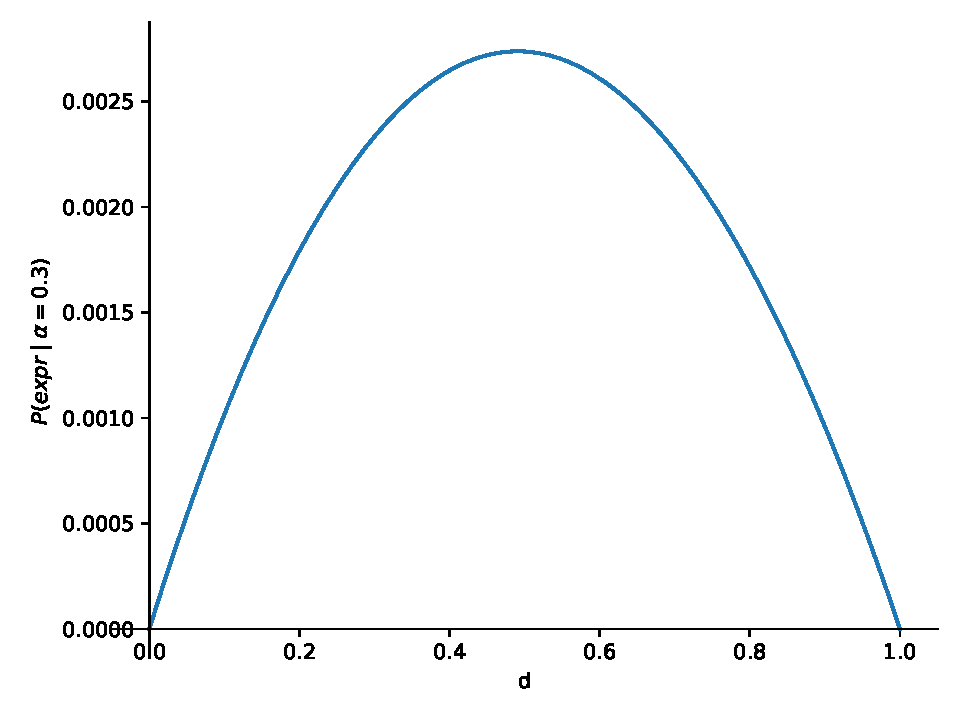
\includegraphics[height=15em]{Pabc_alpha03.pdf}
        \end{center} 
        
        \item If a data set $E$ entails \emph{e.g.} $\pr{abc \mid E} = 0.0015$ we can numerically solve
        $$
        \begin{aligned}
            \pr{abc \mid x = 0.3} &= \pr{abc \mid E} \cr
            \iff\cr
            \frac{0.09 d \del{d - 1}}{0.09 d^{2} - 0.69 d - 7.9} &= 0.0015
        \end{aligned}
        $$
        which has two solutions, $d \approx 0.15861$ or $d \approx 0.83138$.
    \end{itemize}
\end{frame}
% ================================================================
\subsection{Non-stratified programs}
% ================================================================
\begin{frame}
    The following LP is non-stratified, because has a cycle with negated arcs:
    $$
    \begin{aligned}
        c_1 &= a\lor \neg a,\cr
        c_2 &= b \larr \naf c \land \naf a, \cr
        c_3 &= c \larr \naf b.
    \end{aligned}
    $$    
    This program has three stable models
    $$
    \begin{aligned}
    s_1 &= \set{ a, c }, \cr
    s_2 &= \set{ \neg a, b }, \cr
    s_3 &= \set{ \neg a, c }.
    \end{aligned}
    $$
\end{frame}

\begin{frame}    
    The disjunctive clause $a\lor\neg a$ defines a set of \textbf{total choices}
    $$
    \Theta = \set{
        \theta_1 = \set{ a },
        \theta_2 = \set{ \neg a }
    }.
    $$
\end{frame}
% ================================================================
\begin{frame}
    
    Looking into probabilistic events of the program and/or its models, we define $x = \pr{\Theta = \theta_1}\in\intcc{0, 1}$ and $\pr{\Theta = \theta_2} = \co{x}$.
    
    Since $s_1$ is the only stable model that results from $\Theta = \theta_1$, it is natural to extend $\pr{ s_1 } = \pr{\Theta = \theta_1}  = x$. However, there is no clear way to assign $\pr{s_2}, \pr{s_3}$ since \emph{both models result from the single total choice} $\Theta = \theta_2$. Clearly, 
    $$\pr{s_2 \mid \Theta} + \pr{s_3 \mid \Theta} =
    \begin{cases}
        0 & \text{if}~\Theta = \theta_1\cr
        1 & \text{if}~\Theta = \theta_2
    \end{cases}
    $$
    but further assumptions are not supported \emph{a priori}. So let's \textbf{parameterize} the equation above,
    $$
    \begin{cases}
        \pr{s_2 \mid \Theta = \theta_2} = &\beta \in \intcc{0, 1} \cr
        \pr{s_3 \mid \Theta = \theta_2} = &\co{\beta},
    \end{cases}
    $$
    in order to explicit our knowledge, or lack of, with numeric values and relations.
\end{frame}
% ================================================================
\begin{frame}
    Now we are able to define the \textbf{joint distribution} of the boolean random variables $A,B,C$:
    
    $$
    \begin{array}{cc|l}
        A, B, C& P & \text{Obs.}\cr
        \hline
        a, \neg b, c & x & s_1, \Theta=\theta_1\cr
        \neg a, b, \neg c & \co{x}\beta  & s_2, \Theta=\theta_2\cr
        \neg a, \neg b, c & \co{x}\co{\beta} & s_3, \Theta=\theta_2\cr
        \ast & 0&\text{not stable models}
    \end{array}
    $$
    where $x, \beta\in\intcc{0,1}$.
\end{frame}
% ================================================================
\section{Conclusions}
% ================================================================
\begin{frame}
    \begin{itemize}
        \item We can use the basics of probability theory and logic programming to assign explicit \emph{parameterized} probabilities to the (stable) models of a program.
        \item In the covered cases it was possible to define a (parameterized) \emph{family of joint distributions}.
        \item How far this approach can cover all the cases on logic programs is (still) an issue \emph{under investigation}.
        \item However, it is non-restrictive since \emph{no unusual assumptions are made}.
    \end{itemize}
\end{frame}
% ================================================================
\section*{ASP \& related definitions}
% ================================================================
\begin{frame}
    
    \begin{itemize}
        \item An \deft{atom} is $r(t_1, \ldots t_n)$ where
        \begin{itemize}
            \item $r$ is a $n$-ary predicate symbol and each $t_i$ is a constant or a variable.
            \item A \deft{ground atom} has no variables; A \deft{literal} is either an atom $a$ or a negated atom $\neg a$.
        \end{itemize}
        
        \item An \deft{ASP Program} is a set of \deft{rules} such as $h_1 \vee \cdots \vee h_m \leftarrow b_1 \wedge \cdots \wedge b_n$.
        \begin{itemize}
            \item The \deft{head} of this rule is $h_1 \vee \cdots \vee h_m$, the \deft{body} is $b_1 \wedge \cdots \wedge b_n$ and each $b_i$ is a \deft{subgoal}.
            \item Each $h_i$ is a literal, each subgoal $b_j$ is a literal or a literal preceded by $\naf\;$ and $m + n > 0$.
            \item A \deft{propositional program} has no variables.
            \item A \deft{non-disjunctive rule} has $m \leq 1$; A \deft{normal rule} has $m = 1$; A \deft{constraint} has $m = 0$; A \deft{fact} is a normal rule with $n = 0$.
        \end{itemize}
        
        \item The \deft{Herbrand base} of a program is the set of ground literals that result from combining all the predicates and constants of the program.     
        \begin{itemize}
            \item An \deft{event} is a consistent subset (\emph{i.e.} doesn't contain $\set{a, \neg a}$) of the Herbrand base.
            \item Given an event $I$, a ground literal $a$ is \deft{true}, $I \models a$, if $a \in I$; otherwise the literal is \deft{false}.
            \item A ground subgoal, $\naf b$, where $b$ is a ground literal, is \deft{true}, $I \models \naf b$, if $b \not\in I$; otherwise, if $b \in I$,  it is \deft{false}.
            \item A ground rule $r = h_1 \vee \cdots \vee h_m \leftarrow b_1 \wedge \cdots \wedge b_n$ is \deft{satisfied} by the event $I$, \emph{i.e.} $I \models r$, iff 
            $$
            \forall j \exists i~I \models b_j \implies I \models h_i.
            $$
            \item A \deft{model} of a program is an event that satisfies all its rules. Denote $\fml{M}_P$ the set of all models of $P$.
        \end{itemize}
        
        \item The \deft{dependency graph} of a program is a digraph where:
        \begin{itemize}
            \item Each grounded atom is a node.
            \item For each grounded rule there are edges from the atoms in the body to the atoms in the head.
            \item A \deft{negative edge} results from an atom with $\naf\;$; Otherwise it is a \deft{positive edge}.
            \item An \deft{acyclic program} has an acyclic dependency graph; A \deft{normal program} has only normal rules; A \deft{definite program} is a normal program that doesn't contains $\neg$ neither $\naf\;$.
            \item In the dependency graph of a \deft{stratified program} no cycle contains a negative edge.
            \item \textbf{A stratified program has a single minimal model} that assigns either true or false to each atom.
        \end{itemize}
        \item Every \emph{definite program} has a unique minimal model: its \deft{semantic}.
        \item Programs with negation may have no unique minimal model.
        \item Given a program $P$ and an event $I$, their \deft{reduct}, $P^I$, is the propositional program that results from
        \begin{enumerate}
            \item Removing all the rules with $\naf b$ in the body where $b \in I$.
            \item Removing all the $\naf b$ subgoals from the remaining rules.
        \end{enumerate}
        \item A \deft{stable model} (or \deft{answer set}) of the program $P$ is an event $I$ that is the minimal model of the reduct $P^I$.  
        \item Denote $\fml{S}_P$ the set of all stable models of program $P$. The \deft{semantics} (or \deft{answer sets}) of a program $P$ is the set $\fml{S}_P$.
        \begin{itemize}
            \item Some programs, such as $a \leftarrow \naf a$, have no stable models.
            \item A stable model is an event closed under the rules of the program.
        \end{itemize}
    \end{itemize}
\end{frame}
% ================================================================
\end{document}